\documentclass[a4paper]{scrartcl}
\usepackage[utf8]{inputenc}
\usepackage[english]{babel}
\usepackage{graphicx}
\usepackage{lastpage}
\usepackage{pgf}
\usepackage{wrapfig}
\usepackage{fancyvrb}
\usepackage{fancyhdr}

\usepackage[font=footnotesize,labelfont=bf,skip=2pt]{caption}
\usepackage{hyperref}

\pagestyle{fancy}

% Create header and footer
\headheight 27pt
\pagestyle{fancyplain}
\lhead{\footnotesize{Data Storage Paradigms, IV1351}}
\chead{\footnotesize{Project Report, Task 1}}
\rhead{}
\lfoot{}
\cfoot{\thepage\ (\pageref{LastPage})}
\rfoot{}


\title{Project Report, Task 1}
\subtitle{Data Storage Paradigms, IV1351}
\author{Vincent Ferrigan ferrigan@kth.se}
\date{\today}

\begin{document}
\maketitle
    
% \section*{Tips for Report Writing}
% \textbf{REMOVE THIS SECTION BEFORE SUBMITTING THE REPORT.}\\

% \noindent \textit{The target audience has exactly the same skills as the author,
% except they do not know anything at all about the specific application described
% in the report.} \\

% Consider the following:

% \begin{itemize}
%   \item \textbf{The report must be \textit{centered around the requirements}.
%   Which are they (Introduction), how did you work to meet them (Method), what is
%   the solution that meets them (Result), and how can you be sure they are met
%   (Discussion). This is the IMRaD method.} The requirements on the Introduction,
%   Method, Result and Discussion chapters are described below under each chapter.

%   \item Is spelling and grammar correct? Is spoken language avoided?

%   \item Does the report have a good structure with sections, subsections and
%   paragraphs?

%   \item Is the text clarified with images and/or other figures, and with links
%   to the code in your Git repository? Remember that all figures (images, tables,
%   graphs, code listings, etc) shall be numbered and have a short explaining
%   text.
% \end{itemize}

\section{Introduction}
The assignment involved creating a 
\emph{conceptual model} 
for the 
\emph{Soundgood music school} 
database. 
A conceptual model is a model that only describes the parts of the reality that
are to be stored in the database.
It includes the main concepts (entities) required to store
information and the relationships that exist between these entities.
The conceptual stage is, however, only an initial model, without all the details required to
create a database. 

This model is the first type of Entity-Relation Diagram (also called ER diagram or
ERD) introduced in the course. 
ER diagrams are used for all types of database
models.  
In this report, the ER diagram was modelled using \emph{Crow's foot notation}
-- also known as Information Engineering notation (IE).

The author collaborated with
\emph{Elin Blomquist}
when constructing the conceptual model described in this report.

% \textbf{This chapter tells \textit{what} are you going to do.} 

% Explain the task and the requirements on the solution. It's important to clearly
% state the requirements. \textit{Also specify which other student you worked with
% when solving the tasks, or if you worked alone.} 

\section{Literature Study}
% This chapter must prove that you collected sufficient knowledge before starting
% development, instead of just hacking away without knowing how to complete a
% task. State what you have read and briefly summarize what you have learned.

% EB:
% Higher grade:
% You will have to read about inheritance first (for example in the text book),
% since it is not much covered in the lectures. 
The pre-recorded lectures on both domain and conceptual models, given by the
course examiner, were reviewed, and chapters three and four in the main textbook
(Fundamentals of Database Systems) as well as sections 6.1-6.4 in the
alternative textbook (Database System Concepts) were examined. 
Additionally, the document 
\href{https://canvas.kth.se/courses/43013/files/7095362?wrap=1}{tips-and-tricks-task1.pdf}
was studied.

\section{Method}
\label{sec:method}
% \textbf{This chapter tells \textit{how} you solved the task.}

% Explain how you worked when solving the tasks and how you evaluated that your
% solution met the requirements. \textit{Do not explain your solution and do not
% refer to code}, that belongs to the \textit{Result} chapter. More specific
% instructions for the content can be found under each task on the Project page in
% Canvas.

% \textbf{EB:}
% - mention which diagram editor you used
% - explain the procedure you followed to create the conceptual model
% - you shall mention all steps that are covered in the videos on conceptual modeling. NO RESULTS
% - If you did not perform a particular step, explain why the result was better (or at least not worse) without that step. 

% The "steps" in question: 
% 1. Noun identification - find all nouns in the specification and make them
% into entities
% 2. Use a category list - get inspired from the category list and creative,
% make entities out of all relevant things that are related to any of the
% existing entities.
% 3. Remove unnecessary entities
% 4. Find attributes - string, boolean, number, time. Can not have attributes
% themselfs. Not a part of an entity.
% 5. Find all associations 
% 6. Review - redo any of the steps above if necessary 

% When doing these steps for a conceptual model, focus on data and relations.
% Some guidelines are: 
% - No entity without attributes
% - Important to find all attributes
% - Define cardinality for  all attributes, and if it is allowed no value
% - Important to find all relations, and decide their cardinality

% While making the entities, we only focused on non-identifying attributes,
% according to the instruction. 
This section outlines the systematic approach taken to develop the conceptual
model for 
\emph{The Soundgood music school} 
database system, represented through an
ERD using crow's foot notation.

\subsection*{Tools}
The modeling tool used was \emph{PlantUML}.
PlantUML is an open-source tool for creating diagrams using a text-based
syntax.
It was chosen to enable version control through git and to avoid using a
proprietary graphical editor.
This report was also written in plain text mode -- \LaTeX.

All code was written in \emph{Visual Studio Code}.
Quick-fixes and editing was, however, done in \emph{Vim}.

\subsection*{The overall Work-flow}
The following steps were taken in order to create the conceptual model based on
the project description 
and the above mention pre-recorded lectures on the topic.

\begin{description}
  \item[Step 1: Noun Identification] 
  The initial step involved an examination of the provided specifications to
  identify potential entities. Every noun was considered a candidate entity,
  under the assumption that nouns typically represent objects within the system,
  which could either be physical (e.g., 'Instrument') or conceptual (e.g.,
  'Enrollment'). Please note that some of these candidates may be converted
  to attributes in the later process of modeling (see step 4).

  \item[Step 2: Category List] To enrich the entity list and ensure no vital
  element was overlooked, a category list was employed. This list helped to
  identify additional potential entities that may not have been immediately
  evident from the noun identification step.
  
  The category list in question, can be found in the provided lecture videos or
  in the book ''A First Course in Object Oriented Development, chapter 4''
  (REF).

  \item[Step 3: Entity Evaluation: Removing Unnecessary Entities or duplicates]
  Following the collation of entities, an evaluation was conducted to eliminate
  redundancies and non-essential or non-relevant entities.

  \item[Step 4: Attribute Determination]
  When examining the entities identified in the previous steps, the focus
  shifted to determining which of them were truly entities and which would be
  better represented as attributes of other entities. 
  The primary guideline was atomicity, i.e., attributes must be indivisible to
  remain meaningful. 
  An attribute should represent the most granular piece of data that is of
  interest to the system (e.g. a string, boolean, timestamp etc.).

  Furthermore, if an identified entity did not possess attributes, it signaled a
  need for reassessment of its role within the model. Entities without
  attributes are seen as potential indicators of misclassification, as each
  entity must encapsulate data through attributes to contribute value to the
  conceptual model.

  Entities that could not meet this criterion were either reclassified as
  attributes or removed from the model. 

  \item[Step 5: Association Mapping]
  The inter-entity relationships were then defined, creating a network of
  associations. Each association was examined to understand its nature
  (dependencies) and cardinality.

\item[Step 6: Model Review and Iteration]
  An iterative review was done to make sure that entities, attributes, and their
  associations were complete and accurate. This cyclical process allowed the
  model to be improved, so it was in line with the systems requirements.
  
  The guidelines followed during this cyclic development process was as follows
  \begin{description}
    \item[Entity Attribution:]
    Every entity was required to have at least one attribute. This rule
    prevented the inclusion of empty or non-informative entities within the
    model.

    \item[Cardinality Specification:]
    Cardinalities for all attributes were defined, including constraints on
    whether null values were permissible. 

    \item[Relation Identification:]
    Identifying all relevant relationships and their cardinalities between
    entities. This included defining whether the relationships were one-to-one,
    one-to-many, or many-to-many, ensuring clarity in the data structure.

    \item[Non-Identifying Attributes:]
    In accordance with the video instructions, the focus was placed exclusively
    on non-identifying attributes. Identifying attributes that could serve as
    primary or candidate keys in a database is done in
    \emph{the Logical and Physical Model}.
  \end{description}
\end{description}

\pagebreak
\section{Result}

% \textbf{This chapter explains \textit{the result} of what you did.}

% \textbf{The report must show that you have done the work yourself and that you
% have understood what you have done}, both of these goals are met by carefully
% explaining your solution here in the result chapter, and proving that it meets
% the requirements. \textit{State each requirement that is met} and explain
% \textit{how you met it}. Also include links to your code in your Git
% repository, and include also diagrams, see Figure \ref{fig:diag}, and other
% figures to illustrate your reasoning. All figures must be referenced in the
% text. Ask yourself if the solution is clearly explained, and if the reader
% will understand the application. What would you yourself want to know if you
% read about the application, is that included in the report? More specific
% instructions for the content can be found under each task on the Project page
% in Canvas. 

% EB:
% - show and briefly explain your conceptual model.

% Higher grade: 
% - Also show how the same relation could be modeled without using inheritance.
% The Result chapter of the report must include one conceptual model diagram
% with inheritance, using the inheritance symbol, and one diagram that models
% the same thing without inheritance. 

\begin{figure}[h!]
  \begin{center}
    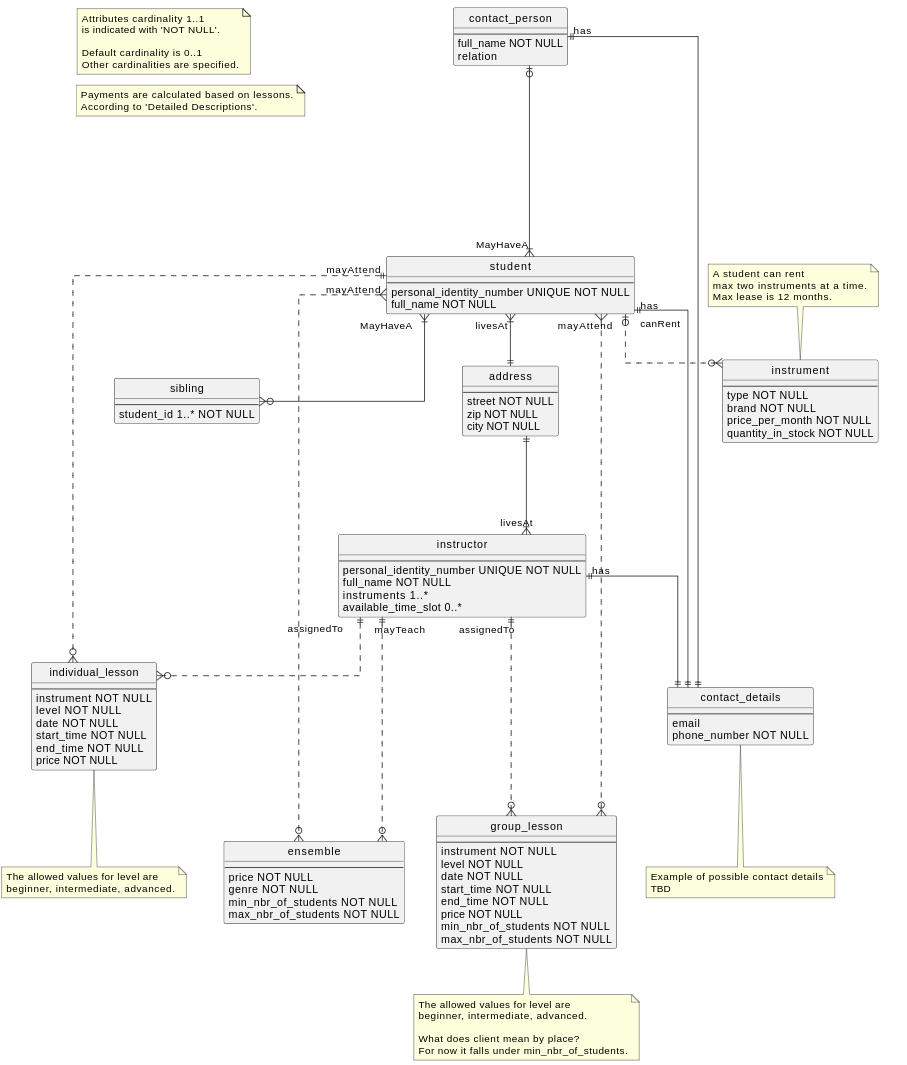
\includegraphics[width=\textwidth]{figures/c_model.png}
    \caption{The Conceptual Model drawn as an ERD using IE notation}
    \label{fig:diag}
  \end{center}
\end{figure}
A couple of notes are used to clarify cardinality restriction, which were chosen
not to be modelled to avoid clutter. 
The \verb|level| attribute, included in the 
\verb|group_lesson| and 
\verb|individual_lesson|
entities, is an enumeration (enum) of the skill-levels 
\verb|beginner|, 
\verb|intermediate|
and 
\verb|advanced|.
The naming convention is based on 
Mozilla's SQL Style Guide. 

Therefore, \emph{Snake Case}
(sometimes referred to as underscore case or 
 snake\_case)
is used, where each space is replaced with underscore
and all letters, including the first letter, is written in lowercase. 

\section{Discussion}
The model, illustrated in figure \ref{fig:diag}, was constructed with maximum
data integrity in mind.
Pricing schemes and data relating to tasks, performed by the school
administration, were therefore avoided, since it can be based on derived data.
Administrative staff are regarded as users, while the booking system or
interface is regarded as a distinct system from the database and are therefore
not included in this initial model. One could further argue that they are part
of the application that handles the operations and/or user interface, rather
than being part of a database.  
On the other hand, the interface and other things left-out (like e.g.
admin-entities) could have been referred to as a note in the diagram.  

Even though there are open issues (described below), the project group considers
the conceptual model to contain all the necessary data to complete the first
project task.  

\subsubsection*{Atomicity}
As mentioned in the chapter \ref{sec:method} (Method) 
attributes must be indivisible to
remain meaningful i.e. atomicity.
The attributes
level
\verb|full_name|
are therefore questionable.

The handling of name attributes was considered. 
For enhanced adaptability,  it
would be better to divide the 
\verb|full_name| into ''first\_name'' and ''last\_name'' or
possible even adding an optional attribute for ''middle\_name'' 
This approach helps with various functions, such as querying specific
individuals based on a last name, or organizing lists.

A full name can easily be assembled from its parts, 
whereas breaking down a full
name into individual components is not as straightforward. 
For example,
personalizing an email with ''Dear [First Name]'' 
is simple when the first name is
stored separately, but challenging when only a full name is available.

Despite these advantages, the group opted to merely specify the presence of a
''full name'' attribute in the conceptual model, postponing the decision to split
the name until later stages of development to maintain flexibility.

\subsubsection*{Places}
In the project description, under the subsection lesson, it states 
\emph{''A group lesson has a specified number of places...''}. 
This statement is ambiguous,
and further clarification would have been needed. It could either mean the
number of accepted students or the number of locations. The project group
decided to use the former, even though discussions were held on which case to
use,  or both to be on the safe side.  In the project description, there is a
section that says the model can't have things that aren't in the detailed
description.

\subsubsection*{Other possible entities and attributes}
\begin{figure}[h!]
  \begin{center}
    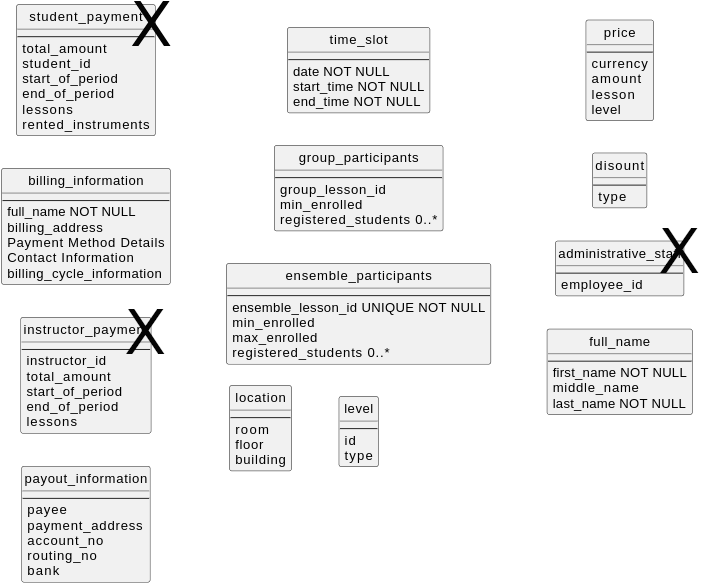
\includegraphics[width=0.7\textwidth]{figures/e_cand.png}
    \caption{Other entity candidates discussed}
    \label{fig:e_cand}
  \end{center}
\end{figure}
The project group chose to add some attribute examples in the entity 
\verb|contact_details|,
(with a note that these
are only examples of possible contact details) and 
must therefore be discussed 
with the client. 

From the category list one can identify a possible entity
called ''classroom'' (location).
The project group chose not to include it, 
since the project description never explicitly required 
the database system to keep track of where lessons took place.
Something one naturally could add to the client-discussion. 

Other possible entities would be a ''time slot'', grouping 
together the attributes
\verb|date|
\verb|start_time|
\verb|end_time|.

\subsection*{Possible inheritance}
Many of the entities share common properties. 
Inheritance can therefore be applied to the model. 
For example, 
ensemble, 
\verb|group_lesson| and 
\verb|individual_lesson| 
all share common attributes, such as 
\verb|price|
\verb|level| and 
\verb|date|. 
(Furthermore, 
\verb|group_lesson| and 
\verb|individual_lesson| share attributes instruments)

These attributes can be grouped together
in a parent entity called lesson, session or booking. 
The sub-entities will then only include attributes that are more
unique to them. 
Such as the attribute
\verb|genre|.

The same technique can be used with the 
\verb|instructor| and 
\verb|student|,
who all can inherit common properties from a 
person 
parent entity. 
Attributes in common are 
\verb|personal_identify_number| and 
\verb|full_name| 
and are further linked to the dependent entities 
\verb|contact_details|
and 
\verb|address|.


% \textbf{This chapter \textit{analysis} the result presented in the previous section.} 

% Evaluate your solution according to the assessment criteria found in the assessment-criteria documents, which are found under the bullet \textit{In the Discussion chapter of your report...}, under each task on the Project page in Canvas. You do not have to cover all specified criteria.

% EB:
% ˆ Does the CM contain all information needed by Soundgood?
% ˆ Is it easy, that is a reasonable number of hops, to collect information related to all of the major entities (student, lesson, instructor, etc).
% ˆ Does the CM have a reasonable number of entities? Are important entities missing? Are there irrelevant entities, for example entities without attributes?
% ˆ Are there attributes for all data that shall be stored? Do all attributes have cardinality? Is the cardinality correct? Are the correct attributes marked as NOT NULL and/or UNIQUE?
% ˆ Does the CM have a reasonable number of relations? Are important relations missing? Are there irrelevant relations? Does all relations have cardinality at both ends and name at least at one end?
% ˆ Are naming conventions followed? Are all names sufficiently explaining?
% ˆ Is the notation (UML or crow foot) correctly followed?
% ˆ Are all business rules and constraints that are not visible in the diagram explained in plain text?
% ˆ Is the method and result explained in the report? Is there a discussion? Is the discussion relevant?

% Higher grade:
% - The report must include a relevant and extensive Discussion chapter about the mandatory part of the task.
% - Discuss advantages of using inheritance and advantages of not using inheritance. 


% Discission: 
% - Levels, are they entity of attribute? Why did we decide to make a note out of it? 
% - Bookings: patr of an interface? 
% - Price is based on a lesson, which is unique in its existance.
% - Name: decided "full-name", because what is a name? In this stage, it is only relavant that it exists. 

% * Kontaktuppgifts tabell med personID som aktörerna är kopplade till. Eller en
%   supertyp PERSON som aktörerna "subtypas" ifrån. 
% * PersonID, StudentID, InstruktörsID bytas ut mot personnummer:
%     * Förenklad lösning
%     * Personnummer är unikt
%   Men en kontaktpersons personnummer är ju irrelant så nej

% * With inheritance duplicate contact information is stored for persons that are both instructors and students. 
% Perhaps, person can be switched to contact_detail/contact_info?
% or one can use person_id. 

% JOINT "person" with contact details. A person has a contact ID and can be a contact person, student and/or instructor. No duplicats. The person has an ID.

% Contact-details för studenter, instruktörer och contact person. Contact person ska inte ha personnumber och address!!!!!

% * **id** -> system generated. "person number" (a.k.a. personnummer, social security nbr) should not be a requirement for ICE

% * **name-issue** -> You can always construct a full name from its components, but you can't always deconstruct a full name into its components
% ' https://www.kalzumeus.com/2010/06/17/falsehoods-programmers-believe-about-names/
% ' https://stackoverflow.com/questions/1122328/first-name-middle-name-last-name-why-not-full-name 

% * **ensemble** -> Should it be a subtype of lesson-parent (the parent for group and individual) or its own?  The instructions separate them.

% * A group lesson has a specified nbr of places (which may vary) -- WHAT DOES THAT MEAN?
% Enbart ensemble har maximium? Men places i group betyder max? Eller?
%   - Ska den då har en egen "entity"??
% * ska minimum nbr of students logiken vara med i en dB?
% * Ska genre och level vara egna entities eller typ enums?
% * Finns fixed time slots och non fixed schedual för privata lektioner. Är det något som ska speglas i dBn?

% * Admin staff? Ska det vara en database eller via en "app providing a user interface"---dvs bokningssystem

% Bookings entity instead of lessons!! Eller ska lessons vara en parent och bookings något separat.

% One price for beginner and intermediate, and one for advanced. -- Men kommer det alltid att gälla? Inte bra för flex. Vidare står det att they might not always
% have the same price for beginners and intermediate lessons

\end{document}